\documentclass[tikz,border=8pt]{standalone}
\begin{document}
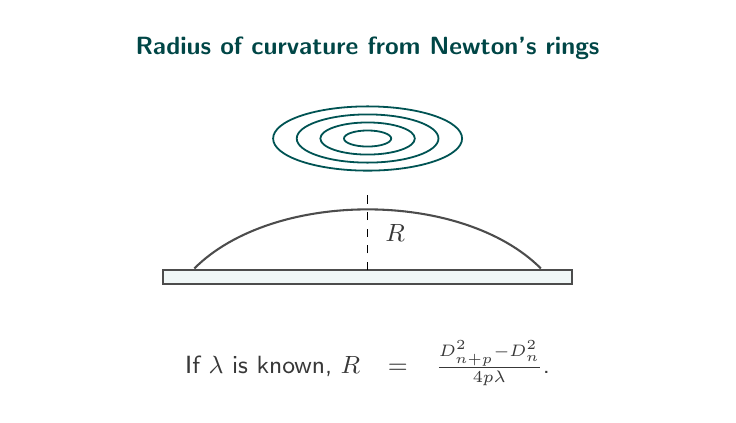
\begin{tikzpicture}[
  line/.style={draw=black!70,line width=0.75pt},
  label/.style={font=\sffamily\small,text=black!78},
  title/.style={font=\sffamily\bfseries\small,text=teal!55!black},
]
\node[title] at (0,3.0) {Radius of curvature from Newton's rings};
\draw[line,fill=teal!6] (-2.6,0) rectangle (2.6,0.18);
\draw[line] (-2.2,0.2) .. controls (-1.2,1.2) and (1.2,1.2) .. (2.2,0.2);
\draw[dashed] (0,0.18)--(0,1.15);
\node[label,right] at (0.1,0.65) {$R$};
\foreach \r in {0.30,0.60,0.90,1.20}{
  \draw[teal!65!black,line width=0.65pt] (0,1.85) ellipse ({\r} and {0.34*\r});
}
\node[label,align=center,text width=8.4cm] at (0,-1.0)
  {If $\lambda$ is known, $R=\frac{D_{n+p}^2-D_n^2}{4p\lambda}$.};
\end{tikzpicture}
\end{document}
